\chapter{Introducción}

En Mayo de 2001, la ARIB (Association of Radio Industries and Businesses)\cite{ARIB} presentó la primera versión de su estándar para la transmisión de televisión digital. Coloquialmente denominada ``Norma Japonesa de Televisión Digital", académicamente ISDB-T, por sus siglas en inglés provenientes de \textit{Integrated Services Digital Broadcasting, Terrestrial}. La norma sintetiza un conjunto de requerimientos técnicos para la utilización eficiente del espectro radioeléctrico para la transmisión de datos multimedia, con la colaboración y el aval de todos los actores de la industria, como proveedores de tecnología, compañías de broadcasting, investigadores del área, entre otros.

Esta norma basa muchos de sus conceptos en la norma DVB-T, publicada por primera vez en el año 1997 por la organización europea DVB (Digital Video Broadcasting). La posterioridad de ISDB-T con respecto a ésta permitió que se robustecieran algunos de los aspectos más criticados de la norma europea, resultando en un estándar mas robusto para la transmisión. Discutiremos algunos de estos aspectos mas adelante, cuando se presente la norma en el capitulo 3.

Actualmente, existen en el mundo cuatro grandes estándares comerciales. Además de ISDB-T y DVB-T, están la norma china DTMB (Digital Terrestrial Multimedia Broadcast) y la norma norteamericana de la ATSC (Advanced Television Systems Comitee). La elección de qué norma adoptar por parte de los gobiernos nacionales radica exclusivamente en decisiones políticas, cuyo análisis y discusión escapan a los objetivos de este documento.

En Uruguay, al igual que en gran parte de Latinoamérica, se adoptó en 2011 una versión de ISDB-T denominada ISDB-T International, la cual es a grandes rasgos idéntica a la primera, salvo por algunos cambios menores como el cambio en la codificación de fuente (pasa del estándar MPEG-2 a MPEG-4) y la elección de otro estándar de interactividad (se cambia de BML a Ginga).

Luego de la adopción del estándar, en el decreto 585/12 del Ministerio de Industria Energía y Minería (MIEM) se fijó el 21 de Noviembre del año 2015 como la fecha limite para el denominado ``apagón analógico"\cite{decreto_apagon}, fecha en la cual se dejaría de transmitir televisión por vías analógicas, pasando exclusivamente a medios digitales, liberando los espectros asignados para los canales de TV abierta para otros fines. 

Durante la implementación del marco legal de la nueva norma de televisión digital se entregaron 22 licencias para transmisión de contenidos bajo la norma ISDB-T International (en adelante ISDB-T por simplicidad). Al día de hoy, tres años después de la fecha limite para el apagón, solo algunos de los actores del rubro están brindando el servicio de forma adecuada y llama la atención la baja participación del sector comercial en la transformación analógico-digital. La asignación de bandas de frecuencia para los proveedores del servicio de televisión abierta, quedo trunco luego de disputas comerciales, en un fallo del Tribunal de lo Contencioso Administrativo (TCA), que dejo sin efecto el decreto 585/12 \cite{cancelacion_decreto_apagon}. En esa sentencia, queda también sin efecto la aplicación del apagón analógico, lo que probablemente colaboro con la desaceleración de la transformación tecnológica por parte de los canales comerciales.

Relevamos la situación de las estaciones de transmisión de televisión digital a lo largo del país, mediante una consulta que elevamos a la Dirección Nacional de Telecomunicaciones (DINATEL). En la figura \ref{mapa_estaciones} presentamos un mapa con las estaciones activas al día de hoy. Hemos encontrado que la cobertura abarca solo una parcialidad del territorio nacional, existiendo incluso departamentos del interior del país que aún no tienen cobertura en su totalidad.

\begin{figure}
	\centering
	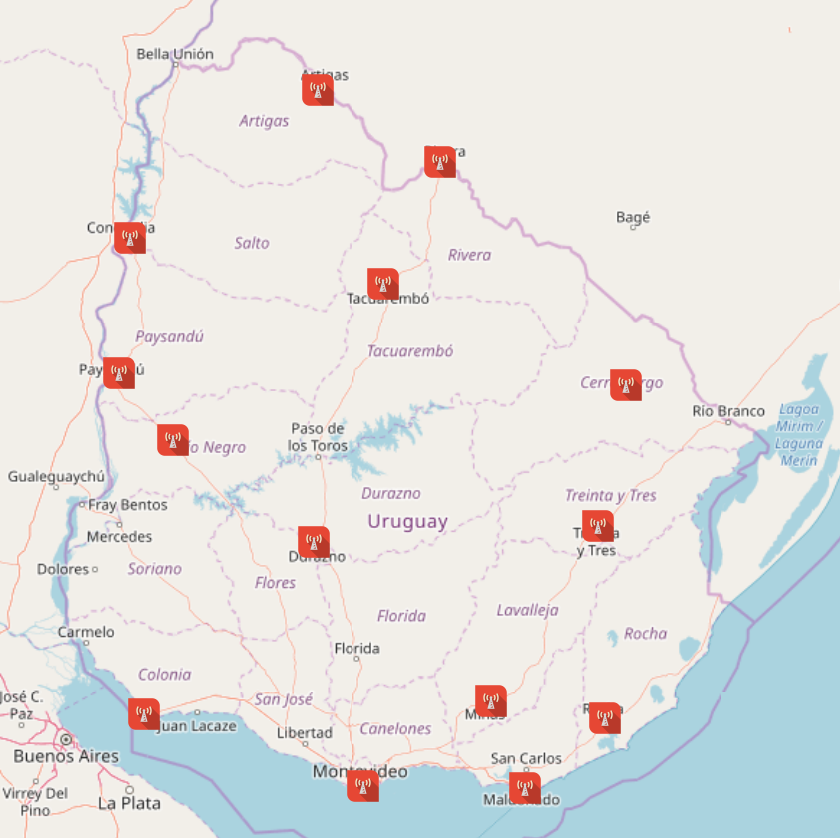
\includegraphics[scale=0.3]{figuras/cap01/mapa_estaciones}
	\caption{\label{mapa_estaciones} Distribución de las estaciones transmisoras de TV digital en el Uruguay.}
\end{figure}

La situación de los consumidores del servicio también dista de la ideal, pues la televisión analógica sigue siendo la mayor puerta de acceso al medio. La Encuesta Continua de Hogares del Instituto Nacional de Estadística\cite{ine2017}, cuyos indicadores son una muestra representativa de la situación de todos los hogares del país, dió a conocer que en el año 2017 una reducida parte de los hogares encuestados tienen recepción de TV digital abierta. Tanto es así, que el apagón analógico fue pospuesto por tiempo indeterminado luego del mencionado fallo del TCA. El alto costo del recambio de equipamiento, posturas sobre la democratización del acceso a la información para personas de bajos recursos, fundamentan estas decisiones.

Durante el auge de la TVD, en los momentos posteriores a la adopción de la norma, surgió la necesidad de generar documentación técnica para la implementación de la misma. Mediante una colaboración entre la DINATEL y la Facultad de Ingeniería, se desarrollo el proyecto \textit{gr-isdbt} \cite{winCom16}. Pablo Belzarena, Pablo Flores, Gabriel Gómez, Víctor González-Barbone y Federico La Rocca presentaron un receptor de televisión digital, de código abierto y bajo el paradigma de radio definida por software (SDR, paradigma de transmisión que explicaremos en detalle más adelante).

Nuestro proyecto complementa el trabajo iniciado en \textit{gr-isdbt}, pues con la implementación del transmisor ISDB-T, se completa el sistema de transmisión de televisión digital de punta a punta. Ambos trabajos en conjunto permiten visualizar y ayudan a comprender el funcionamiento del sistema presentado en la norma, teniendo acceso completo a todo lo que sucede dentro del mismo, en cualquier punto de la cadena de transmisión y recepción. 

Además, genera la posibilidad de recrear una planta de transmisión de televisión a muy bajo costo, permitiendo su implementación tanto en el hogar por entusiastas, en el aula por docentes o en la industria, por técnicos, lo cual puede colaborar con el mejoramiento de la calidad del servicio actual. A su vez, puede servir incluso como ejemplo para algunos de los cursos de la Facultad, generalmente catalogados por el estudiantado como muy teóricos y con poco alcance práctico. 

Implementar un transmisor de televisión digital no es una tarea sencilla. El primer problema a enfrentar es el acceso a la información técnica. Existe poca documentación generada en el país para cumplir con las condiciones técnicas de un sistema complejo y que, además, ya lleva 7 años de vigencia como oficial. La norma presentada por la ARIB deja varias zonas grises, asume por conocidos conceptos clave, y no se explaya más de lo necesario en cuestiones de fondo. 

También existen fuertes limitaciones económicas para hacerse con software o hardware comercial que resuelvan incluso algunas de las funcionalidades más básicas que exige la norma. 

Esta tesis intenta resolver ambas, complementando el trabajo iniciado por el grupo ARTES con el receptor \textit{gr-isdbt}. Se desarrolló a lo largo de este proyecto, un transmisor de televisión digital que cumple con las condiciones establecidas en la norma, y cuyas señales son decodificables por los televisores comerciales homologados por el LATU. El resultado es la posibilidad de implementar a pequeña escala y por un costo considerablemente menor, un sistema funcional de transmisión de TVD. Además, presentamos en este documento, un análisis de la norma y explicamos de qué forma se resolvieron los problemas de implementación y de las zonas "poco claras" que se mencionaron antes.

Contar con el trabajo presentado en \textit{gr-isdbt} fue de una ayuda mayúscula, ya que disponer del código completo del receptor ayudó a comprender, sintetizar y testear los conceptos teóricos vertidos en la norma, lo que fue fundamental para la comprensión de las funcionalidades que sería necesario implementar para poder transmitir. 

Para este grupo de trabajo es importante destacar lo valioso de la existencia de proyectos de código abierto. Incontables veces encontramos en la comunidad puntos de vista, ideas y hasta algoritmos para resolver los problemas encontrados en el camino. Es por eso que esperamos poder contribuir con ella, poniendo a disposición de cualquier persona el transmisor \textit{gr-isdbt-tx}, para que continúen con el trabajo de aprendizaje y la optimización del mismo por técnicos y estudiantes, seguramente con un mejor panorama del rubro, que el que tuvimos al implementar este proyecto.

Esperamos también, mediante el desarrollo de este documento, poder contribuir con la comunidad nacional de técnicos que trabajan en el rubro, y que no cuentan con documentación técnica generada por y para la norma nacional, con los problemas y las particularidades que la transmisión tiene en nuestro país y no tener que abstraer de trabajos de terceros, que resolvieron problemas similares en contextos diferentes. Entendemos que en este proyecto, los conceptos desarrollados por la norma se sintetizan en órdenes básicas al procesador, y al ser de código abierto y gratuito, se democratiza el acceso a una información a la que hoy por hoy solo se accede por medio de hardware y software propietario con licencias de costos elevados.

Para esta documentación, que acompaña el código presentado para el transmisor, definimos seis capítulos en los que se explica el desarrollo del mismo. En el capitulo 2 presentamos algunos de los conceptos fundamentales de telecomunicaciones sobre los que se construye la norma. El capitulo 3 realiza un breve pasaje por los puntos clave del sistema transmisor ISDB-T, los cuales son necesarios para comprender algunos de los bloques que conforman el sistema. Para profundizar más en los mencionados conceptos, invitamos al lector a revisar la tesis de maestría de Pablo Flores, que pueden encontrar en \cite{gr-isdbt}. Luego, el capitulo 4 se detiene particularmente en el concepto de radio definida por software y  presenta en detalle una implementación del mismo, en particular aquel sobre el cual se desarrolló el transmisor, que es GNU Radio en conjunto con un equipo USRP. En el capitulo 5 analizamos el código generado para implementar el transmisor, explicando en cada paso los conceptos del capitulo 2 y 3 que se necesita aplicar en cada bloque, y como se extrapolaron a C++, lenguaje en el que se escribió cada uno de los bloques de procesamiento. Mas adelante, en el capitulo 6 mostramos el desempeño del transmisor como un todo, realizando las evaluaciones practicas del mismo en función de los objetivos de este proyecto y se comentan los resultados obtenidos. Para terminar, en el capitulo 7, presentamos las conclusiones del proyecto en particular y planteamos algunos desafíos que seria interesante afrontar en un futuro.






